\lstset{
  basicstyle=\fontsize{8}{8}\selectfont\ttfamily
}

\subsection{ Main function }
    \lstinputlisting[caption=main.cpp,language=C++]{ ../../linux/linux2/main.cpp }

\subsection{ States machine }
    \lstinputlisting[caption=state.hpp,language=C++]{ ../../linux/linux2/state.hpp }
    \lstinputlisting[caption=state.cpp,language=C++]{ ../../linux/linux2/state.cpp }
        
\subsection{ Registers }
    \lstinputlisting[caption=regs.hpp,language=C++]{ ../../linux/linux2/regs.hpp }
    \lstinputlisting[caption=regs.cpp,language=C++]{ ../../linux/linux2/regs.cpp }

\subsection{ Subroutines }
    \lstinputlisting[caption=tasks.hpp,language=C++]{ ../../linux/linux2/subroutines.hpp }
    \lstinputlisting[caption=tasks.cpp,language=C++]{ ../../linux/linux2/subroutines.cpp }

\subsection{ Terminal }
    \lstinputlisting[caption=terminal.hpp,language=C++]{ ../../linux/linux2/terminal.hpp }
%    \lstinputlisting[caption=terminal.cpp,language=C++]{ ../../linux/linux2/terminal.cpp }

\subsection{ Utils }
    \lstinputlisting[caption=utils.hpp,language=C++]{ ../../linux/linux2/utils.hpp }
    \lstinputlisting[caption=utils.cpp,language=C++]{ ../../linux/linux2/utils.cpp }

\begin{figure}[!htb]
    \centering
    \captionsetup{justification=centering,margin=1.5cm}
    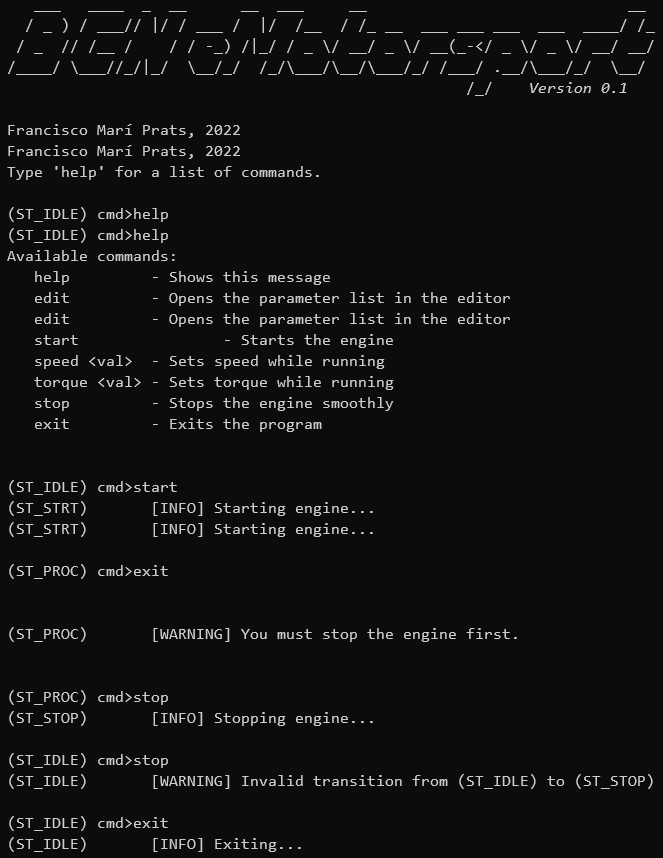
\includegraphics[width=8.5cm]
        { img/5_resultats/interficie.png }
    \caption*{ Prova de la interfície de testeig }
\end{figure}